\documentclass[border=2pt]{standalone}
\usepackage{newtxtext}
\usepackage{tikz}
\usetikzlibrary{positioning,arrows.meta,calc,fit,backgrounds}
\definecolor{corig}{HTML}{D95F02}
\definecolor{ccorr}{HTML}{1B9E77}
\begin{document}
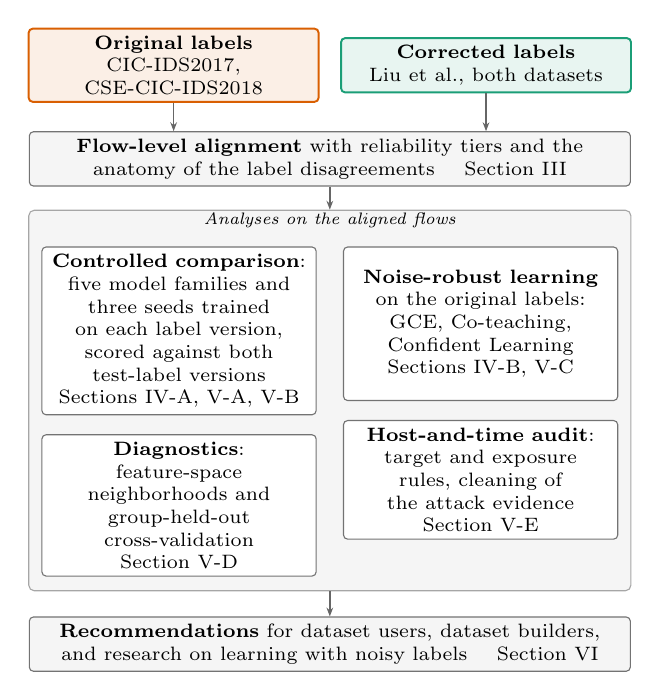
\begin{tikzpicture}[font=\fontsize{7}{8.2}\selectfont,
  every node/.append style={execute at begin node={\hyphenpenalty=10000\exhyphenpenalty=10000\relax}},
  box/.style={draw=black!55, rounded corners=1.5pt, align=center, inner sep=2.6pt, fill=white},
  lab/.style={box, line width=0.7pt},
  arr/.style={-{Stealth[length=3.2pt]}, black!60, line width=0.5pt},
  node distance=4.2mm and 2.4mm]
\node[lab, draw=corig, fill=corig!10, text width=35mm] (orig) {\textbf{Original labels}\\CIC-IDS2017, CSE-CIC-IDS2018};
\node[lab, draw=ccorr, fill=ccorr!10, text width=35mm, right=2.6mm of orig] (corr) {\textbf{Corrected labels}\\Liu et al., both datasets};
\path (orig.south) -- (corr.south) coordinate[midway] (mid);
\node[box, fill=black!4, text width=74.5mm, below=4.2mm of mid] (align) {\textbf{Flow-level alignment} with reliability tiers and the anatomy of the label disagreements \quad Section III};
\node[box, text width=33mm, minimum height=19.5mm, below=7.6mm of align.south west, anchor=north west, xshift=1.6mm] (cmp) {\textbf{Controlled comparison}: five model families and three seeds trained on each label version, scored against both test-label versions\\Sections IV-A, V-A, V-B};
\node[box, text width=33mm, minimum height=19.5mm, below=7.6mm of align.south east, anchor=north east, xshift=-1.6mm] (noise) {\textbf{Noise-robust learning} on the original labels: GCE, Co-teaching, Confident Learning\\Sections IV-B, V-C};
\node[box, text width=33mm, minimum height=15mm, below=2.4mm of cmp] (diag) {\textbf{Diagnostics}: feature-space neighborhoods and group-held-out cross-validation\\Section V-D};
\node[box, text width=33mm, minimum height=15mm, below=2.4mm of noise] (ctx) {\textbf{Host-and-time audit}: target and exposure rules, cleaning of the attack evidence\\Section V-E};
\begin{scope}[on background layer]
\node[draw=black!35, fill=black!4, rounded corners=2pt, inner sep=1.6mm, fit=(cmp)(noise)(diag)(ctx), yshift=1.4mm, inner ysep=3.2mm] (box) {};
\end{scope}
\node[anchor=north, inner sep=1pt, font=\fontsize{6.5}{7.5}\selectfont\itshape] at (box.north) {Analyses on the aligned flows};
\path (diag.south) -- (ctx.south) coordinate[midway] (mid2);
\node[box, fill=black!4, text width=74.5mm, below=7.4mm of mid2] (rec) {\textbf{Recommendations} for dataset users, dataset builders, and research on learning with noisy labels \quad Section VI};
\draw[arr] (orig.south) -- (orig.south |- align.north);
\draw[arr] (corr.south) -- (corr.south |- align.north);
\draw[arr] (align.south) -- (align.south |- box.north);
\draw[arr] (box.south |- box.south) -- (rec.north);
\end{tikzpicture}
\end{document}
